\chapter{Proiectarea și Realizarea Sistemului}
\label{chap:2}

\section{Principiul de Funcționare}

\subsection{Descrierea Funcționării Algoritmului}

Acest algoritm controlează un servo motor %
continuu pentru a gestiona un mecanism %
automatizat de preparare a ceaiului. %
Sistemul include un servo motor care %
bobinează o sfoară, ridicând sau %
coborând un clește ce ține un %
pliculeț de ceai. Utilizatorul poate %
seta durata în care pliculețul de ceai %
rămâne în apă folosind un %
buton albastru. Mai jos sunt descrise %
componentele și funcționalitățile %
principale:

\subsection{Funcționarea Sistemului}

\begin{enumerate}
    \item La pornire, sistemul inițializează %
    \gls{led}-urile și servo-ul în poziția %
    neutră.  

    \item Utilizatorul setează durata de %
    infuzare în minute apăsând %
    butonul albastru, fiecare apăsare %
    adăugând un minut.  

    \item Servo-ul poate fi controlat %
    manual folosind:  
    \begin{itemize}
        \item Butonul alb pentru ridicarea %
        cleștelui (sens orar).  
        \item Butonul roșu pentru coborârea %
        cleștelui (sens antiorar).  
    \end{itemize}

    \item Procesul principal este declanșat %
    prin apăsarea butonului de start, %
    care activează \gls{led}-ul roșu pentru %
    a indica începerea procesului.  

    \item Motorul oscilează inițial pentru %
    calibrare, apoi pliculețul %
    rămâne în apă pentru durata %
    setată, afișând timpul rămas %
    pe consola serială.  

    \item La finalul procesului, cleștele %
    este ridicat automat, iar \gls{led}-ul %
    verde clipeste pentru a semnaliza %
    încheierea operațiunii.  
\end{enumerate}

\subsection{Inițializare Componente}

\begin{itemize}
    \item Se definesc pini pentru \gls{led}-uri, %
    butoane și controlul servo-ului.  

    \item Se configurează intrările și %
    ieșirile în funcția \texttt{setup()}.  

    \item Servo-ul este inițializat într-o %
    poziție neutră (1500 microsecunde).  

    \item \gls{led}-urile sunt setate inițial %
    pentru a indica starea sistemului.  
\end{itemize}

\subsection{Setarea Timpului de Preparare}

\begin{itemize}
    \item \textbf{Butonul albastru (CountButton):} %
    La fiecare apăsare, timpul este %
    incrementat cu un minut.  

    \item \gls{led}-ul alb se aprinde temporar %
    pentru a indica o apăsare validă.  
\end{itemize}

\subsection{Control Manual al Servo-ului}

\begin{itemize}
    \item \textbf{Butonul alb (UpWhiteButton):} %
    Când este apăsat, servo-ul se %
    rotește în sens orar %
    (\gls{pwm} = 1200 microsecunde), ridicând %
    cleștele.  

    \item \textbf{Butonul roșu (DownRedButton):} %
    Când este apăsat, servo-ul se %
    rotește în sens antiorar %
    (\gls{pwm} = 1800 microsecunde), coborând %
    cleștele.  

    \item Când butoanele sunt eliberate, %
    servo-ul este oprit %
    (\gls{pwm} = 1500 microsecunde).  
\end{itemize}

\subsection{Pornirea Procesului Principal}

\begin{itemize}
    \item \textbf{Butonul de start (StartButton):} %
    Inițiază procesul de coborâre a %
    pliculețului de ceai în apă %
    pentru timpul setat.  

    \item \gls{led}-ul roșu se aprinde pentru %
    a indica începerea procesului.  

    \item Servo-ul efectuează o oscilație %
    de 3 cicluri pentru calibrare.  

    \item Procesul principal așteaptă %
    numărul de minute setate %
    (convertit în secunde) și afișează %
    trecerea timpului în consola serială.  

    \item La final, servo-ul ridică %
    cleștele, iar \gls{led}-ul verde %
    clipeste pentru a indica %
    încheierea procesului.  
\end{itemize}

\subsection{Funcții Auxiliare}

\begin{itemize}
    \item \textbf{whiteLed():} Controlează %
    starea \gls{led}-ului alb.  

    \item \textbf{ready\_anim():} Realizează %
    o animație de clipire pentru %
    \gls{led}-ul verde la sfârșitul %
    procesului.  
\end{itemize}


Acest algoritm oferă o soluție automatizată %
și flexibilă pentru prepararea ceaiului, %
permițând utilizatorului să controleze %
durata și mișcarea mecanismului prin %
intermediul butoanelor fizice.




\section{Schema Electrică și Configurația Componentelor}

    \subsection{Schema Electrică}

    \begin{figure}[ht!]
      \centering
      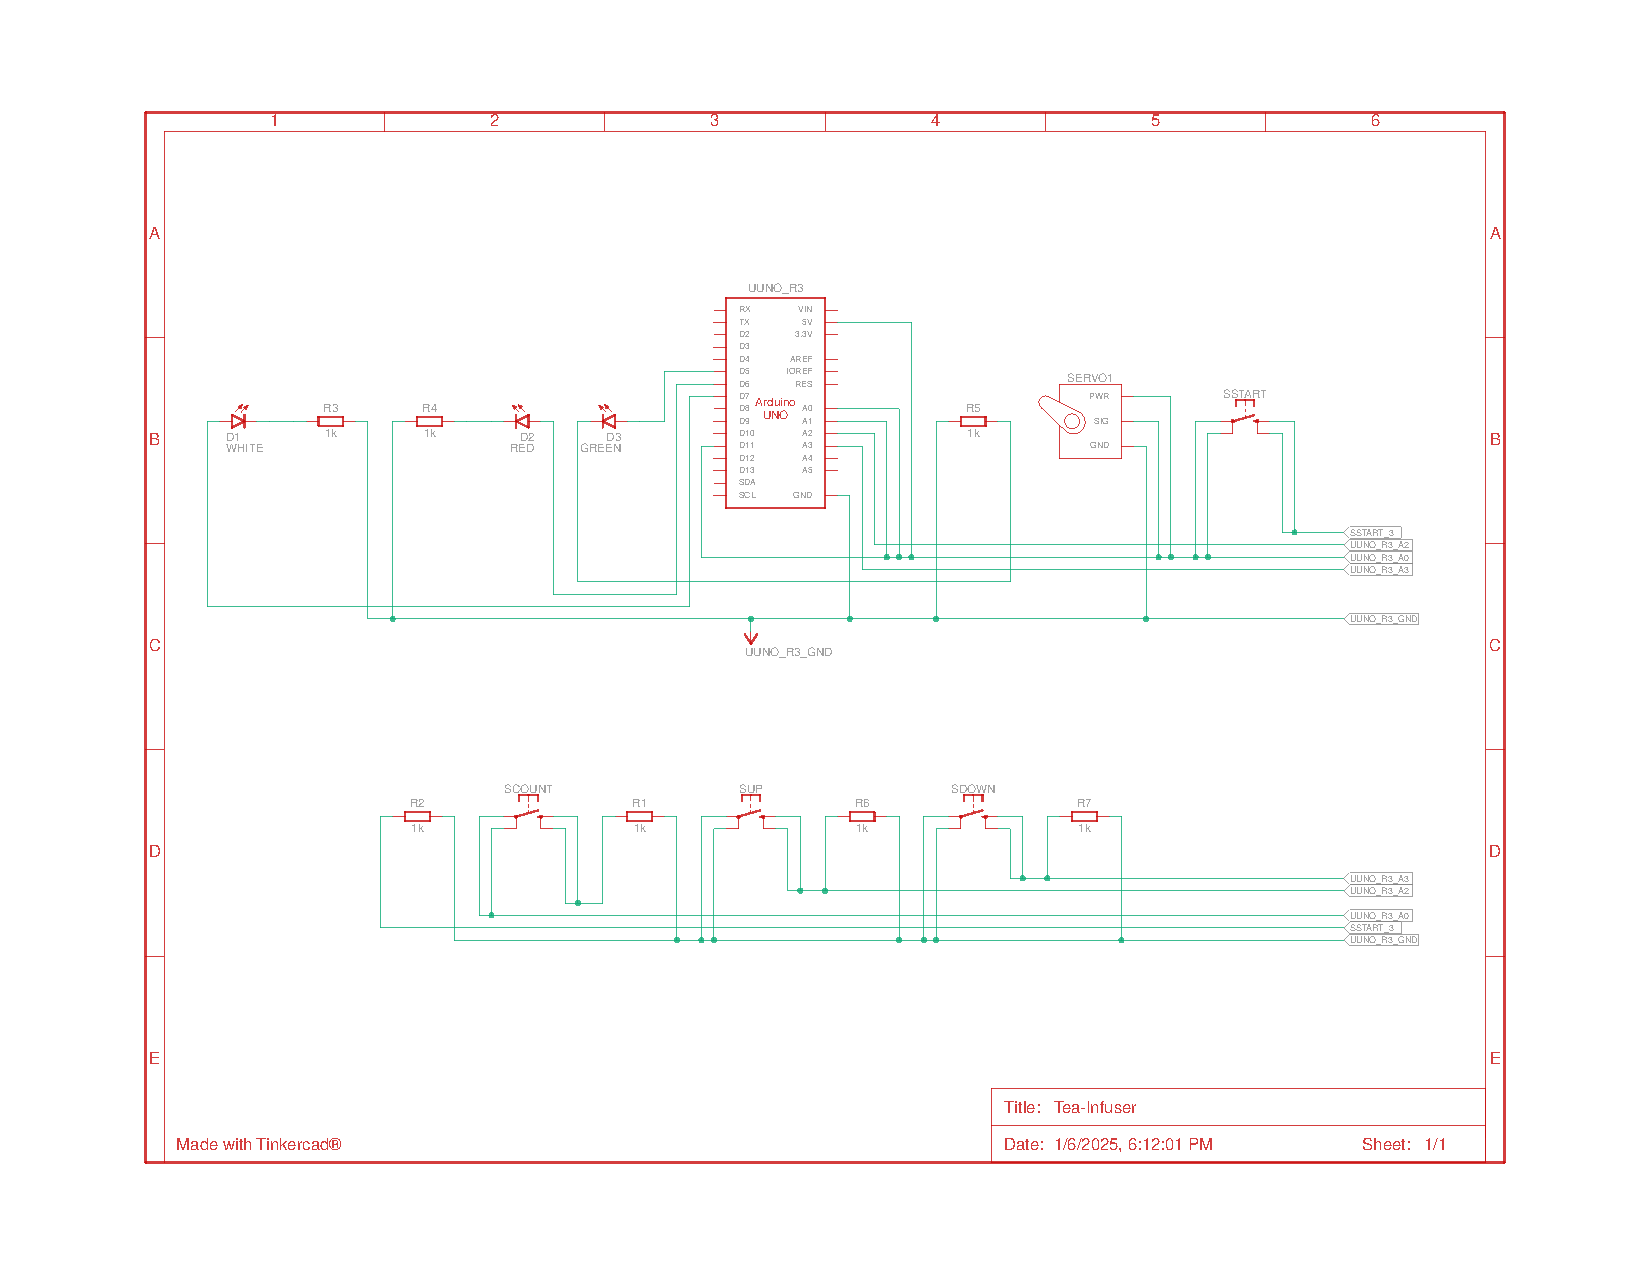
\includegraphics[width=\textwidth]{figures/Schematic.pdf} % Replace 'example.pdf' with your file name
      \caption{Schema Electrică}
      \label{fig:fig1}
    \end{figure}

    \begin{figure}[ht!]
      \centering
      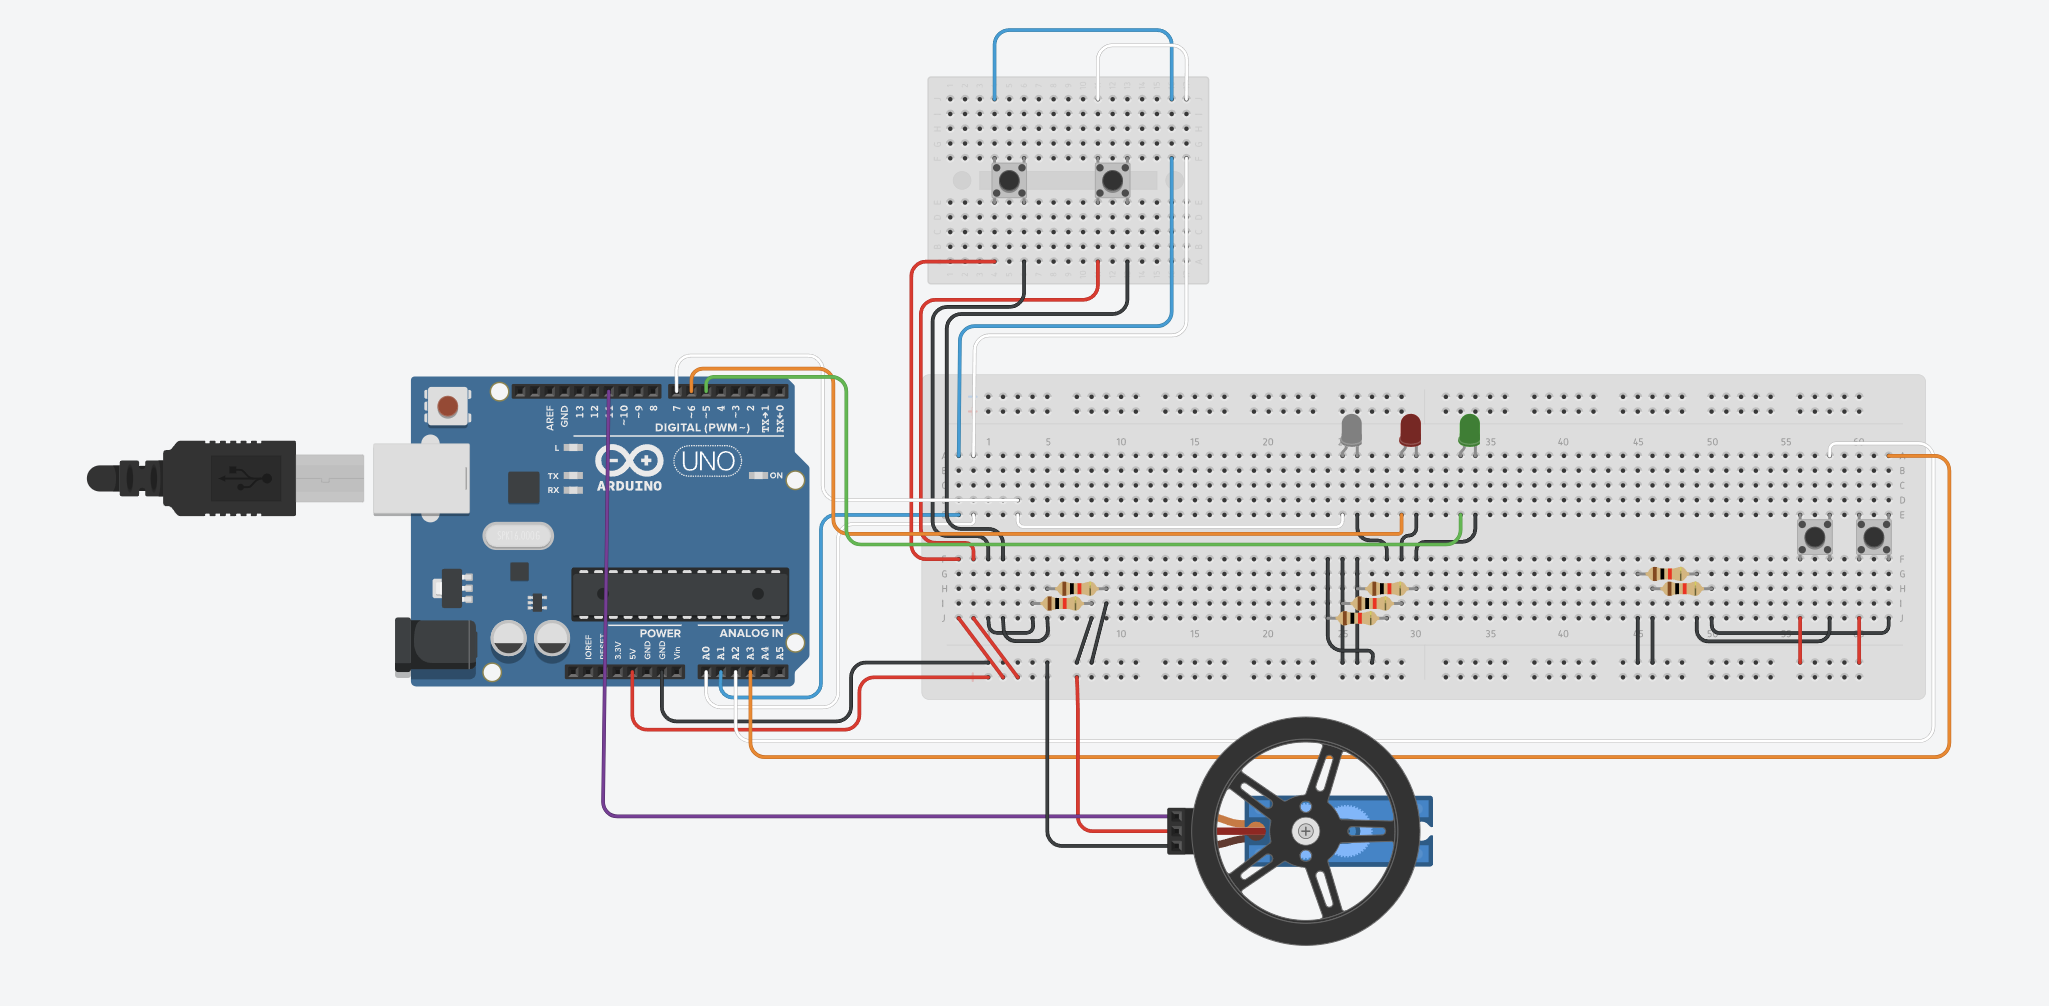
\includegraphics[width=\textwidth]{figures/Circuit.png} % Replace 'example.pdf' with your file name
      \caption{Schemă de Conectare}
      \label{fig:fig2}
    \end{figure}

    \subsection{Configurația Componentelor}
        \begin{itemize}
            \item \textbf{Microcontroler}:  
            Dispozitiv similar cu Arduino UNO R3, %
            bazat pe procesor \gls{atmega} %
            unitatea principală de control. 
            
            \item \textbf{ServoMotor \gls{sg90} 360 grade, continuu}:  
            Utilizat pentru acționarea mecanică a %
            sistemului automatizat.   
    
            \item \textbf{\gls{led}-uri (3 buc.)}:  
              \begin{itemize}
                  \item \gls{led} Verde: Semnalizează abilitatea procesului %
                  de a fi început și terminarea acestuia.  
                  \item \gls{led} Roșu: Semnalizează desfășurarea procesului.  
                  \item \gls{led} Alb: Indică apăsarea de buton pentru a putea %
                  ține cont de numarul de apăsări înregistrate.  
              \end{itemize}
    
            \item \textbf{Butoane (4 buc.)}:  
            \begin{itemize}
              \item Buton Numărător: Incrementează numărul de minute  
              \item Buton Start: Inițiază procesul   
              \item Buton Up: Activează mișcare de ridicare %
              pentru mecanism
              \item Buton Down: Activează mișcare de coborâre %
              pentru mecanism
            \end{itemize}
    
            \item \textbf{Fire de conexiune}:  
            Asigură legăturile electrice între componente.  
    
            \item \textbf{Breadboard}:  
            Utilizat pentru testarea și realizarea conexiunilor provizorii.  
    
            \item \textbf{Baterie externă (2000\gls{mah})}:  
            Baterie externă  cu input 5V/500\gls{mah} și output 5V/1000\gls{mah}, %
            compatibilă cu microcontrolerul și %
            componentele auxiliare pentru funcționarea %
            corectă.   
    \end{itemize}
    



  \section{Probleme Nerezolvate și Motivația Acestora}

    În cadrul proiectului, au fost identificate %
    următoarele probleme nerezolvate, care oferă %
    posibilități de îmbunătățire și dezvoltare %
    ulterioară:
    
    \begin{itemize}
        \item \textbf{Utilizarea senzorilor de greutate:} %
        Sistemul nu include un senzor de greutate %
        pentru a verifica dacă pliculețul de ceai %
        este manipulat corect. Implementarea unui %
        astfel de senzor ar aduce un nivel %
        suplimentar de precizie, dar a fost %
        amânată din cauza constrângerilor de %
        timp și resurse disponibile.  
    
        \item \textbf{Utilizarea senzorilor de poziție:} %
        Lipsa unui senzor de poziție pentru %
        verificarea poziției exacte a %
        pliculețului în timpul manipulării %
        reprezintă o limitare. Un astfel de %
        senzor ar putea îmbunătăți %
        funcționalitatea sistemului prin %
        creșterea acurateței, dar integrarea %
        sa necesită investiții suplimentare %
        în hardware și software.  
    
        \item \textbf{Necesitatea unui senzor de temperatură:} %
        Sistemul nu dispune de un senzor de %
        temperatură pentru monitorizarea apei, %
        ceea ce ar fi util pentru ajustarea %
        automată a timpului de imersiune. %
        Integrarea unui astfel de senzor ar %
        permite optimizarea procesului de %
        preparare a ceaiului, dar această %
        funcționalitate a fost omisă din %
        motive de complexitate și limitări %
        de timp.  
    
        \item \textbf{Conectivitatea cu o aplicație mobilă:} %
        Dispozitivul nu este capabil să %
        comunice cu o aplicație mobilă, %
        deoarece placa utilizată nu dispune %
        de un modul de conectivitate %
        Bluetooth sau Wi-Fi. Această %
        funcționalitate ar fi permis %
        controlul și monitorizarea %
        procesului de la distanță. %
        Integrarea unui modul compatibil %
        necesită componente suplimentare %
        și dezvoltare software avansată.  
    
        \item \textbf{Alimentarea și gestionarea energiei:} %
        Sistemul se bazează pe o baterie %
        externă de 2000\gls{mah}, dar nu a fost %
        testată performanța acesteia pe %
        perioade extinse de utilizare. %
        Monitorizarea consumului și integrarea %
        unei surse de alimentare alternative %
        rămân aspecte de îmbunătățit.  

        \item \textbf{Structura fizică a macaralei:} %
        Structura fizică a macaralei utilizate în acest %
        proiect este una de jucărie, ceea ce limitează aspectul %
        estetic și robustețea acesteia. Utilizarea unei imprimante %
        3D ar fi permis realizarea unui design personalizat, %
        mai atractiv și mai durabil, adaptat cerințelor proiectului.
    \end{itemize}
    
    \bigskip
    
    Problemele identificate în acest proiect %
    subliniază provocările întâmpinate pe parcursul %
    dezvoltării și oferă direcții clare pentru %
    optimizări și îmbunătățiri viitoare.


    

\section{Observații asupra Rezultatelor Obținute}

    Sistemul a demonstrat că poate automatiza %
    procesul de preparare a ceaiului, îndeplinind %
    sarcinile principale pentru care a fost %
    proiectat. Mișcarea mecanismului a fost precisă, %
    iar servo motorul continuu a reușit să %
    înlocuiască eficient motorul \gls{dc} inițial, %
    care nu a avut suficientă putere.  
    
    Testele efectuate au confirmat că dispozitivul %
    funcționează stabil în condiții normale de %
    utilizare. Alimentarea prin baterie a fost %
    suficientă pentru cicluri scurte de operare, %
    dar necesită optimizări pentru utilizarea %
    pe durate mai lungi.  
    
    Butoanele și \gls{led}-urile oferă un sistem de %
    control intuitiv și feedback vizual clar %
    pentru utilizator. Totuși, integrarea unei %
    aplicații mobile ar fi crescut nivelul de %
    utilizare și flexibilitatea dispozitivului.  
    
    În ciuda limitărilor, proiectul a demonstrat %
    fezabilitatea unui sistem automatizat pentru %
    prepararea ceaiului. Rezultatele obținute oferă %
    o bază solidă pentru îmbunătățiri viitoare, %
    atât în ceea ce privește funcționalitatea, %
    cât și aspectul estetic și conectivitatea %
    sistemului.
    




